% Polycopie pour les etudiants

%\documentclass[handout]{beamer}[10pt, usepdftitle=false]
%%\usepackage[printwatermark]{xwatermark}
%\usepackage{pgfpages}
%\pgfpagesuselayout{6 on 1}[a4paper,border shrink=5mm] % 4 par 4

% NE PAS OUBLIER DE BAISSER A QUALITE DU POLYCOPIE!: gs -sDEVICE=pdfwrite -dCompatibilityLevel=1.4 -dPDFSETTINGS=/ebook -dNOPAUSE -dQUIET -dBATCH -sOutputFile=small.pdf big.pdf

% Mes slides pour le cours
\documentclass{beamer}[10pt, usepdftitle=false handout]

\beamertemplatenavigationsymbolsempty

\usepackage[T1]{fontenc}
\usepackage[]{algorithm2e}
\usepackage{multimedia}
\usepackage{gensymb}
\usepackage{textcomp}
\usepackage{array}
\usepackage{fancyvrb}
\usepackage{tabularx,colortbl}

\usepackage{listings}

%\usepackage{background}
%\backgroundsetup{
%    placement=center,
%    scale=5,
%    color=lightgray,
%    contents={PAUL BLONDEL},
%    opacity=0.5
%}
%\setbeamertemplate{background}{\BgMaterial}


%\usepackage[font=small,labelfont=bf]{caption} 

\usetheme{Boadilla}

\title{Introducton to Data Engineering 9}
\author[]{Paul Blondel}
\institute[]{UTSEUS, Shanghai}
\date[]{May 25th, 2021}

\usepackage[style=british]{csquotes}


\def\signed #1{{\leavevmode\unskip\nobreak\hfil\penalty50\hskip1em
  \hbox{}\nobreak\hfill #1%
  \parfillskip=0pt \finalhyphendemerits=0 \endgraf}}

\newsavebox\mybox
\newenvironment{aquote}[1]
  {\savebox\mybox{#1}\begin{quote}\openautoquote\hspace*{-.7ex}}
  {\unskip\closeautoquote\vspace*{1mm}\signed{\usebox\mybox}\end{quote}}


\setbeamertemplate{headline}
{
  \leavevmode%
  \hbox{%
  \begin{beamercolorbox}[wd=1.0\paperwidth,ht=2.25ex,dp=1ex,center]{author in head/foot}%
    \usebeamerfont{author in head/foot}\insertsubsection
  \end{beamercolorbox}}%
  \vskip0pt%
}


\setbeamertemplate{footline}
{
  \leavevmode%
  \hbox{%
  \begin{beamercolorbox}[wd=.5\paperwidth,ht=2.25ex,dp=1ex,center]{author in head/foot}%
    \usebeamerfont{author in head/foot}\insertsection
  \end{beamercolorbox}%
  \begin{beamercolorbox}[wd=.5\paperwidth,ht=2.25ex,dp=1ex,center]{title in head/foot}%
    \usebeamerfont{title in head/foot} \inserttitle \hspace*{2em}  \insertframenumber{} / \inserttotalframenumber\hspace*{2ex} 
  \end{beamercolorbox}}%
  \vskip0pt%
}

\AtBeginSection[]
{
   \begin{frame}
    \tableofcontents[ 
    currentsection] 
   \end{frame}
}

\begin{document}
	{
	\setbeamertemplate{footline}{
  	\leavevmode%
  	\hbox{%
  	\begin{beamercolorbox}[wd=.5\paperwidth,ht=2.25ex,dp=1ex,center]{author in head/foot}%
  	\end{beamercolorbox}%
  	\begin{beamercolorbox}[wd=.5\paperwidth,ht=2.25ex,dp=1ex,center]{title in head/foot}%
  	\end{beamercolorbox}}%
  	\vskip0pt%	
	} 
	\begin{frame}
	\titlepage
	\end{frame}

	\begin{frame}
	
	\begin{aquote}{Dev Ittycheria, President and CEO of MongoDB}
The cost of managing traditional databases is high. Mistakes made during routine maintenance are responsible for 80 percent of application downtime.
	\end{aquote}	
	\end{frame}

	\begin{frame}
		\tableofcontents
	\end{frame}
	}

	\addtocounter{framenumber}{-3}

	\section{Recall}	

    \begin{frame}[label=(first)]
	The main aspects of Relational Databases:
	\vspace*{0.6em}
	
	\begin{itemize}
		\item{Very structured
			\begin{itemize}
				\item{\textbf{Tables}}
				\item{\textbf{Typed attributes}}
				\item{Integrity \textbf{constraints} and \textbf{relations}
					\begin{itemize}
						\item{Uniqueness of \textbf{primary keys} (integrity)}
						\item{Existence of \textbf{foreign keys} (relations)}
						\item{Etc.}
					\end{itemize}					
				}				
			\end{itemize}					
		}
		\item{Can be \textbf{formalized with diagrams}
			\begin{itemize}
				\item{UML, MERISE, etc}
			\end{itemize}					
		}		
		\item{Use \textbf{SQL} language for DB operations}	
	\end{itemize}

	\begin{figure}
	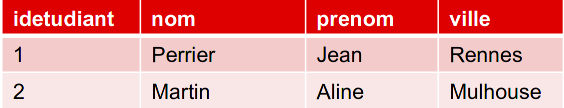
\includegraphics[scale=1.2]{images/sql_example1.png} 
     	\vspace*{-0.5em}
		\caption{SQL example: "SELECT nom,prenom FROM etudiant;}
	\end{figure}
	
	
	\end{frame}

	\begin{frame}
	
	\begin{figure}
	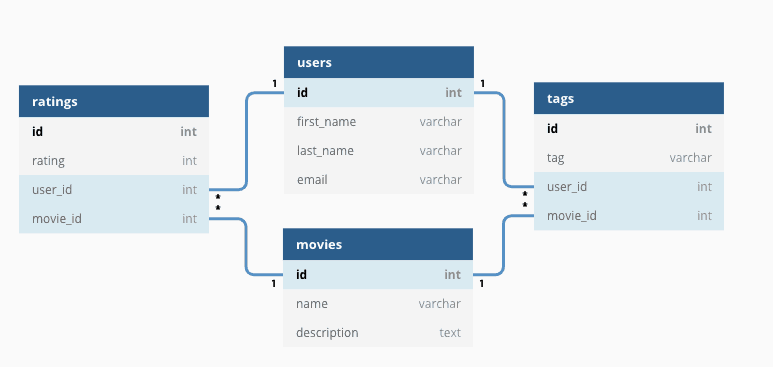
\includegraphics[scale=1.4]{images/db_example1.png} 
     	\vspace*{-0.5em}
		\caption{Example of a relational database diagram}
	\end{figure}
	
	\vspace*{0.6em}	
	
	\begin{itemize}
	\item{There are four tables}
	\item{Each table has a set of typed fields}
	\item{Tables have relations}	
	\end{itemize}		
		
	\end{frame}
	
	\begin{frame}
	
	Relation Databases have pros, and cons...	
	\vspace*{0.6em}	
	
	\begin{itemize}
	\item{Relation Databases are \textbf{difficult to distribute on several servers}}
	\item{They face a \textbf{scaling problem} 
		\begin{itemize}
			\item{A bigger database = a more powerful server = limitations}
		\end{itemize}			
	}	
	\item{They have a \textbf{rigid definition} (schema):
		\begin{itemize}
			\item{Changing the schema is hard (require "migrations" = dangerous)}
		\end{itemize}			
	}
	\item{They are \textbf{slow} (because of all the relations to consider)}
	\end{itemize}

	\end{frame}	
	
	\begin{frame}
		
	A complex Relational Database is hard to maintain...
	\vspace*{0.6em}		
		
	\begin{figure}
	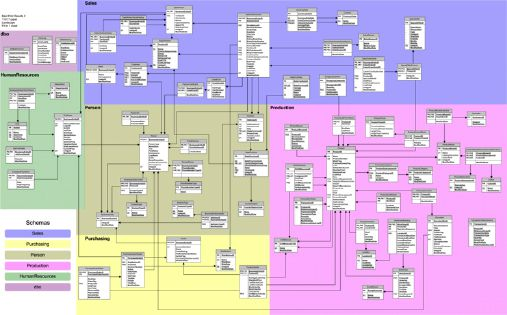
\includegraphics[scale=2.2]{images/example_bigdatabase.png} 
     	\vspace*{-0.5em}
		\caption{Example of a complex Relational Database}
	\end{figure}
	
	
	\end{frame}		
	
	
	\begin{frame}
	
	All these cons make it extremely difficult to deal with Big Data's three Vs...
	\vspace*{0.6em}
	
	\begin{figure}
	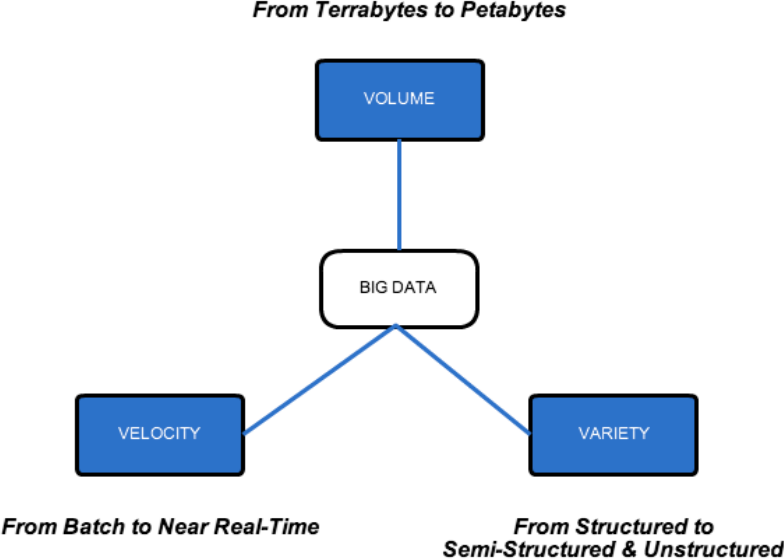
\includegraphics[scale=1.3]{images/three-v.png} 
     	\vspace*{-0.5em}
		\caption{The three Vs.}
	\end{figure}	
	
	
	\end{frame}	
	
	\begin{frame}
	Biggest issue of Relational DB with Big Data is: \textbf{scaling}
	\vspace*{0.6em}
	
	\begin{block}{Why?}
	Relational DB \textbf{cannot easily distribute the storage capacity on other nodes because of the complex relations and constraints} existing between the tables of a relational database 
	\end{block}	
	\vspace*{0.6em}
	
	Indeed, we can only add storage capacity on the same server and also add more processing power (vertical scaling):
	\vspace*{0.6em}	
	
	\begin{figure}
	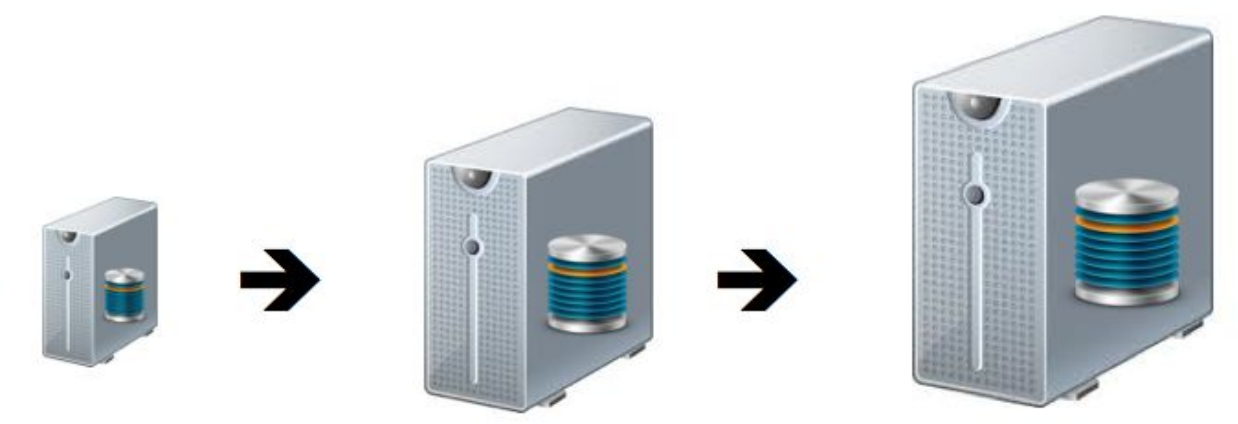
\includegraphics[scale=0.45]{images/vertical-scaling.png} 
     	\vspace*{-0.5em}
		\caption{Vertical scaling of a server containing a Relational DB}
	\end{figure}	
	
	%It is obviously a serious limitation and does not permit to deal with Big Data. Only horizontal scaling permit that. 		
			
	\end{frame}
	
	\section{NoSQL}
	
	\begin{frame}
	
	In the previous course, we saw that \textbf{the way to deal with Big Data is horizontal scaling} (adding nodes in a cluster):
	\vspace*{0.6em}
	
	\begin{figure}
	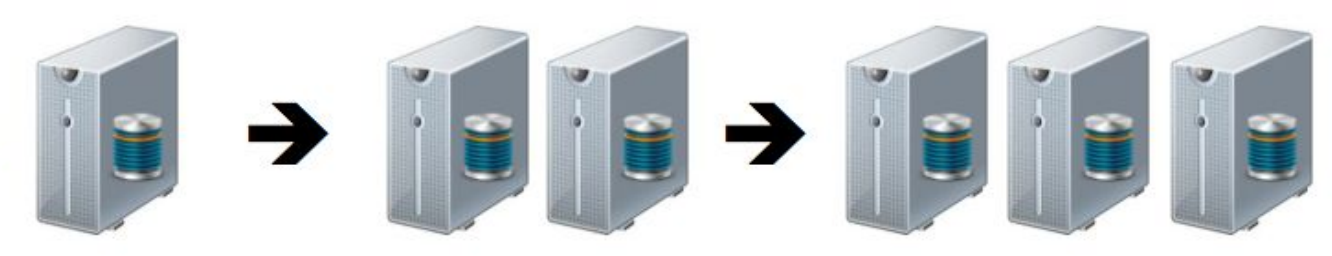
\includegraphics[scale=0.8]{images/horizontal-scaling.png} 
     	\vspace*{-0.5em}
		\caption{Horizontal scaling of a cluster: adding more nodes to increase capacity}
	\end{figure}	
	
	\end{frame}	
	
	\begin{frame}
	
	\begin{itemize}
	\item{Storing data on a cluster of servers and \textbf{benefit from horizontal scaling is possible using NoSQL databases}}
	\item{NoSQL means « Not-Only SQL » and not No SQL (NOTE: some NoSQL databases partially understand SQL)}
	\item{\textbf{NoSQL databases are schemeless}}
	\item{Data can be stored with different scheme on the fly, \textbf{there are no fixed schemes}}
	\item{\textbf{Removing the constraints of Relational DB permits to distribute the DB} on multiples server nodes}	
	\end{itemize}
	
	\end{frame}
	
	\begin{frame}
	
	In a NoSQL database, the information is \textbf{stored as key and value pairs}:
	\vspace{0.6em}

	\begin{figure}
	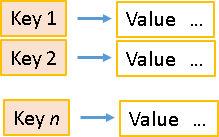
\includegraphics[scale=1.6]{images/key_values1.png} 
	\end{figure}
	
	Example:
	\vspace*{0.6em}	
	
	\begin{figure}
	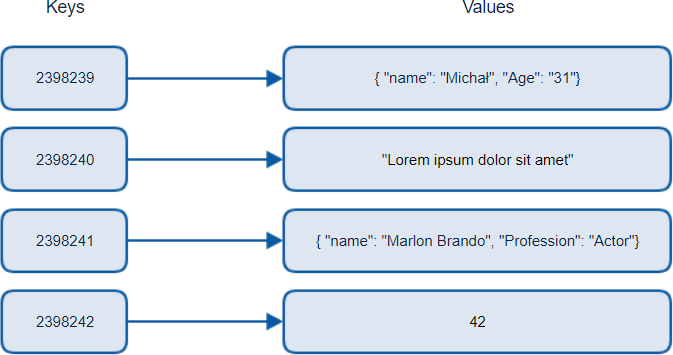
\includegraphics[scale=1.2]{images/key_values2.png} 
     	\vspace*{-0.5em}
		\caption{Contrary to Relational DB, all the information is stored in the "values field" and can be various (JSON, strings, numbers, etc)}
	\end{figure}		
		
	
	\end{frame}
	
	\begin{frame}
	
	A NoSQL database \textbf{can be easily distributed on different nodes of a cluster using of a hash function}:	
	\vspace*{0.6em}

	It is easy to know in which node (or server) is located the data by computing the result of a hash function:
	\vspace*{0.6em}
	
	A hash function is a function \textbf{taking the key in input and giving a number in output which is the node id of the cluster}:	
	\vspace*{0.6em}
	
	Example: HASH(key) → [1 15]
	
	\end{frame}
	\begin{frame}

	%mettre columns gauche et droite icic!

	\begin{columns}[c]
	\column{.4\textwidth}
	\begin{figure}
	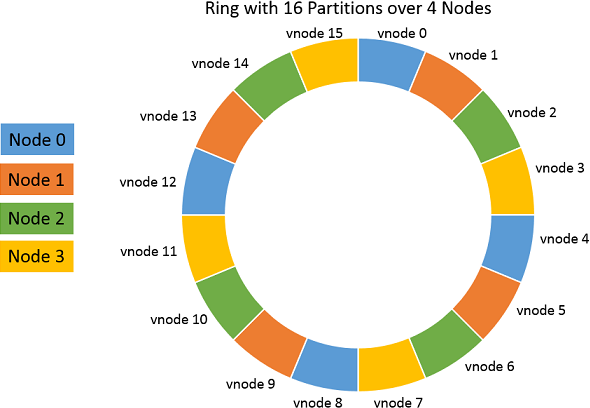
\includegraphics[scale=1.0]{images/vnodes_partition.png} 
	\end{figure}	

	\column{.6\textwidth}
	\begin{itemize}
	\item{Example: we want the values of key 2398239, HASH(2398239)=12. So the values are in the virtual node 12 (a partition of Node 0)}
	\item{Here we have 16 virtual nodes, HASH can be just the modulo of 16 (HASH(X)=X mod 16)}
	\item{If we want to add a new nodes to our cluster: we just have to change the hash function (HASH(X) = X mod 20)}
	\item{Adding nodes to a NoSQL cluster is very easy... It scales horizontally easily.}
	\end{itemize}	
	\end{columns}
	
	\end{frame}	
	
	\begin{frame}

Different types of NoSQL databases, for example:
\vspace*{0.6em}

\begin{itemize}
\item{\textbf{Document DB}: MongoDB, CouchDB, ElasticSearch, etc.}
\item{\textbf{Column DB}: Cassandra, etc.}
\item{\textbf{Key-value purely based}: Redis, etc.}
\item{\textbf{Cache system}: Redis, etc.}
\item{\textbf{Graph}: Neo4j, etc.}
\end{itemize}

	
	\end{frame}	
	
	\begin{frame}
	
	\begin{figure}
	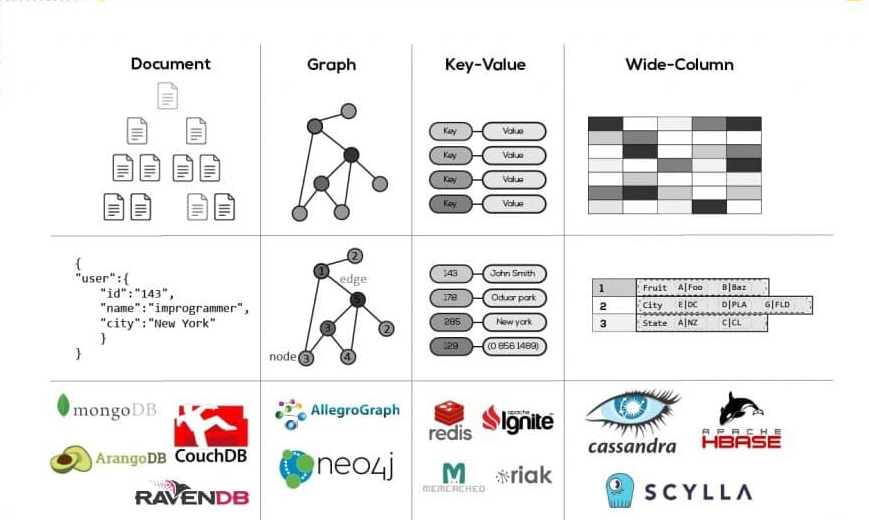
\includegraphics[scale=1.6]{images/nosql_types.png} 
	
	\end{figure}	
	
	\end{frame}
	
	
	\begin{frame}
	
	There are many NoSQL databases but \textbf{no NoSQL standard}	
	\vspace*{0.6em}

	Common points between NoSQL DBs:
	\vspace*{0.6em}
	
	\begin{itemize}
	\item{They have an \textbf{implicit schema}:
		\begin{itemize}
			\item{Data \textbf{schema not predefined on the server side}}
			\item{The \textbf{client application structures the data}}
			\item{Some exceptions: Cassandra V2}
		\end{itemize}			
	}
	\item{There are \textbf{no relations}:
		\begin{itemize}
			\item{No relationship between data or between elements of two collections}
			\item{Some exceptions: Neoj4 and Hive in some cases}
		\end{itemize}				
	}		
	
	\end{itemize}

	\begin{block}{In this course}
	We will see \textbf{MongoDB} and \textbf{ElasticSearch}
	\end{block}
	
	\end{frame}	
	
	\begin{frame}
	
	Advantages and disadvantages of NoSQL and Relational Databases.
	\vspace*{0.6em}

	\textbf{NoSQL}:
	\vspace*{0.6em}

   \begin{itemize}
    \item{\textbf{Advantages}:
    \begin{itemize}
		\item{Can \textbf{deal with large volumes of structured, semi-structured, and unstructured data}}
		\item{Set of \textbf{functions or API easier to use than SQL}}
		\item{\textbf{Efficient horizontal scaling} (instead of expensive vertical scaling)}      
    \end{itemize}
    }
    \item{\textbf{Disadvantages}:
    \begin{itemize}
    	\item{\textbf{Less support} since NoSQL databases are usually open-source}
    	\item{NoSQL databases \textbf{require technical skill} in order to install and maintain}
    	\item{\textbf{Less mature}: they are still growing and many features have to be implemented}
    \end{itemize}
	}
	\end{itemize}	
	\end{frame}
	
	\begin{frame}
	\textbf{Relational databases}:
	\vspace*{0.6em}

	\begin{itemize}
		\item{\textbf{Advantages}:
			\begin{itemize}
				\item{Can \textbf{handle very complex queries, database transactions, and routine analysis of data}}
				\item{Respect "ACID" (\textbf{Atomity}, \textbf{Consistency}, \textbf{Isolation}, \textbf{Durability}): properties ensuring reliable database transactions}
				\item{Can \textbf{handle constraints} (Ex: make sure data can only be deleted if some conditions are met)}
			\end{itemize} 
			}
		\item{\textbf{Disadvantages}:
			\begin{itemize}
				\item{Cannot store \textbf{too complex or too large} images, numbers, designs and multimedia products}
				\item{Can \textbf{become very costly in maintenance and fragile}}
			\end{itemize}				
  	}
	\end{itemize}

	\end{frame}		

	\section{MongoDB: Document based NoSQL}
	
	\begin{frame}
	
	MongoDB: A \textbf{document-based NoSQL database} and the \textbf{most popular NoSQL database}.
	\vspace*{0.6em}
	
	\begin{figure}
	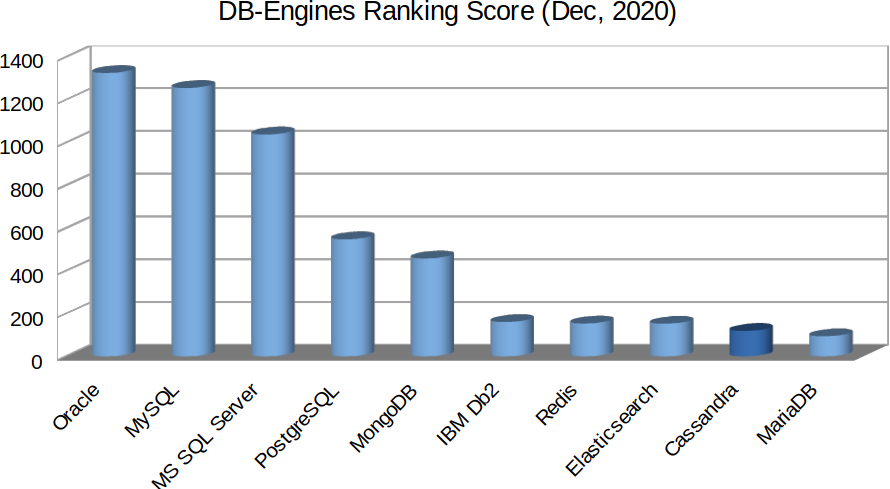
\includegraphics[scale=1.4]{images/db_ranking.png} 
	\end{figure}	
	
	
	\end{frame}
	
	\begin{frame}
	
	\begin{itemize}
		\item{Documents are stored using a \textbf{hierarchical representation}
			\begin{itemize}
				\item{Documents are written with the \textbf{BSON} syntax
					\begin{itemize}
						\item{\textbf{BSON = Binary JSON}}
						\item{BSON: \textbf{extension of the JSON format} containing additional types}	
					\end{itemize}}
			\end{itemize}					
		}
		\item{The DB is \textbf{schemaless}
			\begin{itemize}
				\item{\textbf{No mandatory attribute}}
				\item{\textbf{No fixed type} for an attribute}
				\item{\textbf{No need to perform complex and dangerous DB migrations}}
			\end{itemize}			
		}	
		\item{MongoDB documents are \textbf{similar Python dictionaries} 
			\begin{itemize}
				\item{Set of key/value pairs.}
			\end{itemize}}	
	\end{itemize}

\begin{block}{Note}
Because NoSQL DBs are schemaless, constraints and data relations must be explicitly handled on the application-side.
\end{block}

	\end{frame}

	\begin{frame}[fragile]
	
Example of a BSON MongoDB document:
\vspace*{0.6em}

\begin{verbatim}
{ ‘name’ :’Jean’, ‘height’:170}
{ ‘name’ : ‘Jacques’, ‘height’ : 180, ‘job’ :’teacher’}
{ ‘type’ : ‘car’, ‘brand’ : ‘renault’, ‘price’ : 1500 }
{ ‘type : ‘house’}
\end{verbatim}
	
	\end{frame}
	\begin{frame}
	Properties of MongoDB documents:
	\vspace*{0.6em}
	
	\begin{itemize}
	\item{Keys...
		\begin{itemize}
			\item{are \textbf{string} of characters}
			\item{are \textbf{case sensitives}}
			\item{must \textbf{be unique}: 
				\begin{itemize}
					\item{\{"name": "Romain", "height":185, "name": "Tavenard"\} \textbf{not} valid}	
				\end{itemize}							
			}
		\end{itemize}			
	}
	\item{Values...
		\begin{itemize}
			\item{are \textbf{case sensitives}:  \{"name": "Roman"\} != \{"name": "roman"\}}
			\item{are \textbf{type sensitives}:  \{"height": "185"\} != \{"height": 185\}}
		\end{itemize}			
	}
	
	\end{itemize}
	
	\end{frame}
	\begin{frame}
	
	MongoDB documents are stored in collections \\ (a \textbf{collection = set of documents})
	\vspace*{0.6em}

	\begin{itemize}
		\item{\textbf{Collection}:
			\begin{itemize}
				\item{Example: \lbrack\{"name": "Romain", "height": 185\}, \{"name": "Paul", "height": "172"\}, \{"name": "Romain", "height": 163, "weight\_kg": 65\}\rbrack}
				\item{No schema: keys, values and types can change from one doc to another}	
			\end{itemize}					
		}
	\end{itemize}
\vspace*{0.6em}

Comparison of naming with Relational Databases:
\vspace*{0.6em}

\begin{center}
	\begin{tabular}{ c | c }
\textbf{Relational DB} & \textbf{Document-based DB} \\ \hline
Table &   Collection \\ \hline
Recording & Document	\\ 
	\end{tabular}
\end{center}


\end{frame}	
\begin{frame}

Focus on the \textbf{JSON format}:
\vspace*{0.6em}

\begin{itemize}
\item{Recall: JSON means \textbf{JavaScript Object Notation}}
\item{Example of a JSON document: \{"name": "Romain", "height": 185\}}
\item{Data types:
	\begin{itemize}
	\item{null: \{"x": null\}}	
	\item{Boolean: \{"x": true\}}
	\item{Number: \{"x": 3.14\}}
	\item{String: \{"x": "abcdef"\}}
	\item{Array: \{"x": [1, 5, 7]\}}
	\item{Date: \{"x": new Date()\}}
	\end{itemize}
}
\end{itemize}

\end{frame}	
	
	\begin{frame}
	
How to interogate the DB?
\vspace*{0.6em}

	\begin{itemize}
	\item{\textbf{No need of SQL}}
	\item{Can read/write the DB using \textbf{JavaScript} or \textbf{Python}}	
	\item{Languages allowing more than data access
		\begin{itemize}
			\item{Definition of variables}
			\item{Loops}
			\item{Etc.}	
		\end{itemize}			
	}
	
	\end{itemize}
	
	\end{frame}
	\begin{frame}[fragile]
	How to use MongoDB on Linux:
	\vspace*{0.6em}

Launch the MongoDB deamon (depend on your system).
On GNU/Linux systems using "systemd":
\begin{verbatim}
$ systemctl start mongodb.service
\end{verbatim}

Launch mongo:
\begin{verbatim}
$ mongo
\end{verbatim}

Create a database (or use it, if it already exist):
\begin{verbatim}
> use my_db
\end{verbatim}

Create a collection:
\begin{verbatim}
> db.createCollection("my_collection")
\end{verbatim}

Display the databases:
\begin{verbatim}
> show dbs
\end{verbatim}

Display the collections:

\begin{verbatim}
> show collections
\end{verbatim}
	
	\end{frame}
	\begin{frame}[fragile]
	
We can interrogate MongoDB with Python using the "pymongo" module:
\vspace*{0.6em}

Let's connect to the MongoDB and fetch the database « my\_db » we just created:
\vspace*{0.6em}

\begin{verbatim}
$ python
> from pymongo import MongoClient
> client = MongoClient()
> col = client.my_db
\end{verbatim}
	
	\end{frame}
\begin{frame}[fragile]
Let's see how to perform the basic \textbf{CRUD} operations using pymongo \\
(\textbf{CRUD = Create Remove Update Delete})
\vspace*{0.6em}

\underline{\textbf{Create}}:
\vspace*{0.6em}

Insert a single document using \textbf{insert\_one(document)}:
\begin{verbatim}
> result = col.insert_one({'x':1})
> result.inserted_id
ObjectId('583c16b9dc32d44b6e93cd9b')
\end{verbatim}
 
Insert multiple documents using \textbf{insert\_many(documents)}:
\begin{verbatim}
> result = col.insert_many([{'x': 2}, {'x': 3}])
> result.inserted_ids
[ObjectId('583c17e7dc32d44b6e93cd9c'), 
ObjectId('583c17e7dc32d44b6e93cd9d')]
\end{verbatim}
\end{frame}
\begin{frame}[fragile]
\underline{\textbf{Update}}:
\vspace*{0.6em}

Update a single document matching a filter using \textbf{update\_one(filter, update, upsert=False)}:
\begin{verbatim}
> result = col.update_one({'x': 1}, {'x': 3})
\end{verbatim}
 
Update one or more documents matching a filter using \textbf{update\_many(filter, update, upsert=False)}:
\begin{verbatim}
> result = col.update_many({'x': 1}, {'x': 3})
\end{verbatim}

\end{frame}
\begin{frame}[fragile]

\underline{\textbf{Read}}:
\vspace*{0.6em}

Query the database using \textbf{find(filter=None, projection=None, skip=0, limit=0, no\_cursor\_timeout=False)}: 
\vspace*{0.6em}

The filter argument is a prototype document that all results must match:
\begin{verbatim}
> result = col.find({'x': 1})
\end{verbatim}
 
Get a single document from the collection using \textbf{find\_one(filter=None)}:
\begin{verbatim}
> result = col.find_one()
\end{verbatim}

\end{frame}
\begin{frame}[fragile]
\underline{\textbf{Delete:}}

Delete a single document matching a filter using \textbf{delete\_one(filter)}:
\vspace*{0.6em}

\begin{verbatim}
> result = col.delete_one({'x': 1})
> result.deleted_count
\end{verbatim}

Delete one or more documents matching a filter using \textbf{delete\_many(filter)}:
\begin{verbatim}
> result = col.delete_many({'x': 1})
> result.deleted_count
\end{verbatim}

pymongo also provides \textbf{find\_one\_and\_delete()} and \textbf{find\_one\_and\_replace()} functionality.
\vspace*{0.6em}

\begin{block}{More information}
For more information see the official documentation: 
https://pymongo.readthedocs.io/en/stable/tutorial.html
\end{block}
\end{frame}

\section{ElasticSearch: A different kind of Document-based NoSQL DB}
\begin{frame}
ElasticSearch...
\vspace*{0.6em}

\begin{itemize}
\item{is a different kind of document-based NoSQL database}
\item{is a also powerful \textbf{real-time distributed search and analysis tool}}
\end{itemize}

\vspace*{0.6em}
 
ElasticSearch is used for:
\vspace*{0.6em}

\begin{itemize}
\item{Full text search}
\item{Structured search}
\item{Analysis}
\item{All three combined...}
\end{itemize}
	
\end{frame}
\begin{frame}
ElasticSearch is also a very popular NoSQL DB:
\vspace*{0.6em}

\begin{figure}
	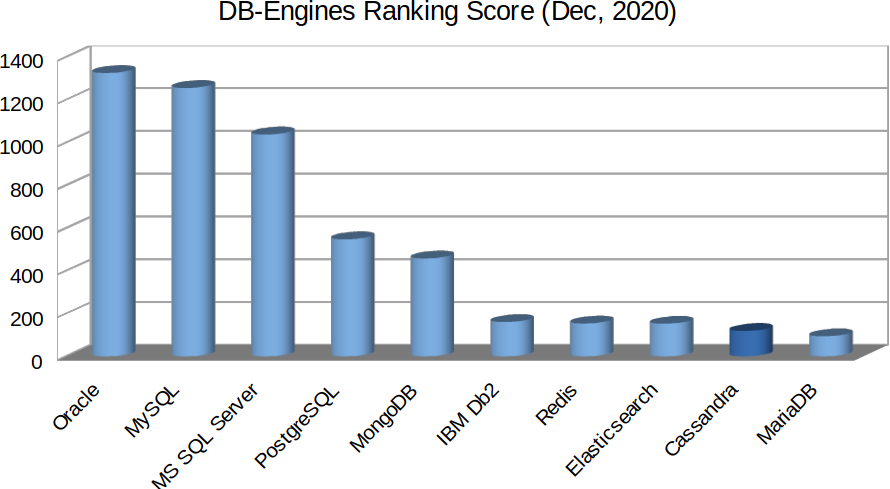
\includegraphics[scale=1.0]{images/db_ranking.png} 
\end{figure}	
\vspace*{0.6em}
	
It is used by:
\vspace*{0.6em}

\begin{itemize}
\item{Wikipedia (http://fr.wikipedia.org)}
\item{The Guardian (http://www.theguardian.com)}
\item{StackOverflow (http://stackoverflow.com/)}
\item{GitHub (https://github.com/)}
\item{Goldman Sachs (http://www.goldmansachs.com/)}
\end{itemize}

\end{frame}

\begin{frame}
ElasticSearch is...
\vspace*{0.6em}

\begin{itemize}
\item{A distributed \textbf{real-time} document DB where \textbf{all fields are undefined and searchable}}
\item{A distributed \textbf{search engine with real-time analysis}}
\item{Capable of supporting a scalability of \textbf{hundreds of servers and petabytes of structured or unstructured data}}
\item{Allow to:
	\begin{itemize}
		\item{Perform and combine \textbf{various searches} on structured, unstructured, geolocation or indicator data}
		\item{\textbf{Explore trends and identify patterns} in the data}
	\end{itemize}
}
\end{itemize}

\begin{block}{Why Elasticsearch?}
Most databases are inadequate at extracting actionable data. They \textbf{cannot do full-text search, handle synonyms, and sort documents by relevance}. Besides, they \textbf{do not do it in real-time}.
\end{block}

\end{frame}

\begin{frame}
How are stored the documents?
\vspace*{0.6em}

\begin{itemize}
\item{The \textbf{content of each document is indexed}}
\item{A document \textbf{has a Type} (which defines its mapping)}
\item{\textbf{Types} are contained in an \textbf{Index}}
\end{itemize}
\vspace*{0.6em}

Comparison ElasticSearch VS Relational Databases VS MongoDB:
\vspace*{0.6em}

\begin{center}
\begin{tabular}{c|c|c|c|c}
Relational DB & Database & Tables & Rows & Columns  \\ \hline
MongoDB & Database & Collections & Documents & Fields  \\ \hline
Elasticsearch & Index & Types & Documents & Fields\\ 
\end{tabular}
\end{center}


\end{frame}
\begin{frame}
Alike MongoDB, \textbf{documents are stored in a cluster}. And we can horizontally scale the cluster by adding nodes:
\vspace*{0.6em}

\begin{figure}
	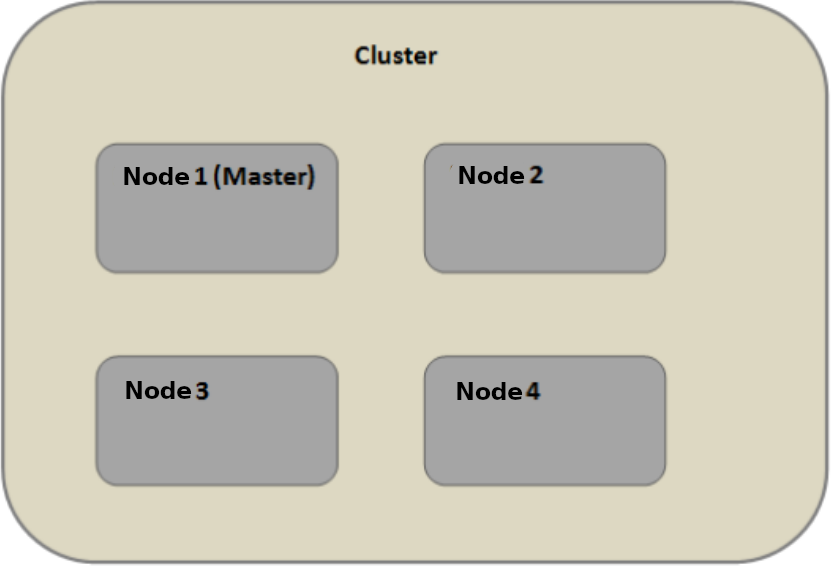
\includegraphics[scale=1.4]{images/elasticsearch_nodes.png} 
\end{figure}	

\end{frame}

\begin{frame}
ElasticSearch is not really a DataBase, \textbf{it is an index}.
\vspace*{0.6em}

\begin{itemize}
\item{An index is a \textbf{logical storage space for documents of the same type} split into one or more Primary Shards}
\item{An index can be \textbf{replicated on zero or more Secondary Shards}}
\end{itemize}

\begin{block}{Shards}
\begin{itemize}
\item{\textbf{Primary Shards}: This is a partition of the index \\ (Default: 5 Primary Shards)}
\item{\textbf{Secondary Shards}: Copies of the Primary Shards \\ (Zero to several times number of Primary Shards)}
\end{itemize}
\end{block}


\end{frame}
\begin{frame}

% Mettre en deux colonnes!!
\begin{columns}[c]
\column{.5\textwidth}

\begin{figure}
	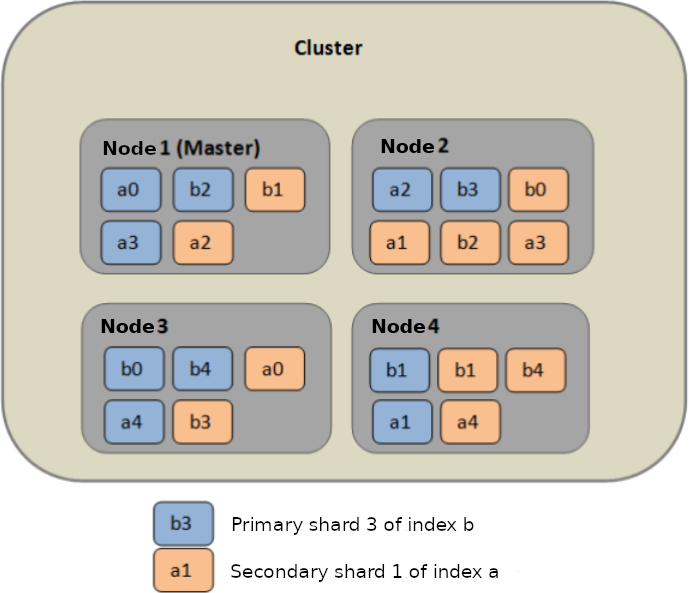
\includegraphics[scale=0.9]{images/elasticsearch_shards.png} 
\end{figure}	

\column{.5\textwidth}
Why we have shards?
\vspace*{0.6em}

\begin{itemize}
\item{It's \textbf{faster to write and read} big amount of data}
\item{It is possible to write on different nodes in the same time, and collect from different locations: \textbf{no funnel effect}}
\item{\textbf{Shards are replicated} to make the cluster more robust}
\end{itemize}
\end{columns}

\end{frame}
\begin{frame}[fragile]

\underline{\textbf{ElasticSearch Document}}
\vspace*{0.6em}

\begin{itemize}
\item{1 document = \textbf{a simple record in an ElasticSearch shard}}
\item{Documents are structured as JSON object and must belong to a \textbf{Type} (defining its structure)}
\end{itemize}
\vspace*{0.6em}

Example:
\begin{verbatim}
{
    "nom": "Paris",
    "codePostal":"75000",
    "monuments": [
        {            
            "nom": "Arc de Triomphe"
        },
        {            
            "nom": "Tour Eiffel"
        }
    ]
}
\end{verbatim}

%\begin{block}{In summary...}
%An ElasticSearch cluster can contain multiple indexes (databases) which, in turn, contain multiple types (tables). These types contain %multiple documents (rows) and each document has properties (columns).
%\end{block}

\end{frame}

\begin{frame}

ElasticSearch offers a \textbf{REST API} to perform operations through HTTP \\ (\textbf{GET, PUT, POST and DELETE methods} can be performed) 
\vspace*{0.6em}

API calls are \textbf{performed on an URL address with the following syntax}: \\
http://localhost:9200/[index]/[type]/[id]/[action]
\vspace*{0.6em}

\begin{itemize}
\item{index: Name of the index}
\item{type: Name of the document type}
\item{id: ID of the document}
\item{action: Action to perform}
\end{itemize}
\vspace*{0.6em}

\begin{block}{Note}
To call the API through HTTP we can use the "curl" command \\ (or Python+requests)
\end{block}

\end{frame}

\begin{frame}[fragile]

Let's see how create an Index named "articles":
\vspace*{0.6em}

\begingroup
\fontsize{6pt}{8pt}\selectfont
\begin{verbatim}
curl -X PUT "localhost:9200/articles?pretty" -H 'Content-Type: application/json' -d'
{
    "settings" : {
        "index" : {
            "number_of_shards" : 3, 
            "number_of_replicas" : 2 
        }
    }
}
\end{verbatim}
\endgroup

And a type:
\begingroup
\fontsize{6pt}{8pt}\selectfont
\begin{verbatim}
curl -XPUT "http://localhost:9200/articles/_doc/_mapping" -d
{
   "_doc": {
      "properties": {
         "title": {
            "type": "string"
         },
         "description": {
            "type": "string"
         },
 	   "author": {
            "type": "string"
         }
      }
    }
}
\end{verbatim}
\endgroup
\end{frame}
\begin{frame}[fragile]
Let's see how to index a document (= insert a document):

\begingroup
\fontsize{6pt}{8pt}\selectfont
\begin{verbatim}
curl -XPOST 'localhost:9200/articles/_doc/1?pretty' -d '{"title": "python tuples",
"description": "practical operations with python tuples","author": "santosh"}' 
-H 'Content-Type: application/json'

This will return :

% Total    % Received % Xferd  Average Speed   Time    Time     Time  Current Dload  Upload   Total   Spent    Left  Speed
100   377  100   222  100   155    222    155  0:00:01 --:--:--  0:00:01  1008{
"_index" : "articles",
"_type" : "_doc",
"_id" : "1",
"_version" : 1,
"result" : "created",
"_shards" : {
"total" : 2,
"successful" : 2,
"failed" : 0
},
"_seq_no" : 0,
"_primary_term" : 1
}

If it succed it will return a HTTP 200 code.
\end{verbatim}
\endgroup
\end{frame}
\begin{frame}[fragile]
Let's see how to delete a document:
\vspace*{0.6em}

\begingroup
\fontsize{6pt}{8pt}\selectfont
\begin{verbatim}
curl -XDELETE 'localhost:9200/articles/_doc/1?pretty'
% Total    % Received % Xferd  Average Speed   Time    Time     Time  Current
Dload  Upload   Total   Spent    Left  Speed
100   241  100   241    0     0    241      0  0:00:01 --:--:--  0:00:01  1928{
"_index" : "articles",
"_type" : "_doc",
"_id" : "1",
"_version" : 2,
"result" : "deleted",
"_shards" : {
"total" : 2,
"successful" : 2,
"failed" : 0
},
"_seq_no" : 1,
"_primary_term" : 1
}
\end{verbatim}
\endgroup

\end{frame}
\begin{frame}[fragile]
And finally an example of a search:
\vspace*{0.6em}

\begingroup
\fontsize{6pt}{6pt}\selectfont
\begin{verbatim}
curl -XPOST "https://localhost:9200/_search" -d'{ "query": { "query_string": { "query": "hello" } } }'  
Results:
{
  "took": 12,
  "timed_out": false,
  "_shards": {
     "total": 12,
     "successful": 12,
     "failed": 0
  },
  "hits": {
     "total": 1,
     "max_score": 0.19178301,
     "hits": [
       {
            "_index": "my-first-index",
            "_type": "message",
            "_id": "AUqiBnvdK4Rpq0ZV4-Wp",
            "_score": 0.19178301,
            "_source": {
                "text": "Hello world!"
                }
            }
        ]
     }
  }
\end{verbatim}
\endgroup
\begin{block}{Official doc}
More information about the Elasticsearch REST API on this website:
https://www.elastic.co/guide/en/elasticsearch/reference/current/docs.html
\end{block}
\end{frame}
\begin{frame}[fragile]
As mentioned above, it's possible to use \textbf{ElasticSearch with Python}:
\vspace*{0.6em}

\begingroup
\fontsize{6pt}{8pt}\selectfont
\begin{verbatim}
settings = {
    "settings": {
        "number_of_shards": 3,
        "number_of_replicas": 2
    },
    "mappings": {
        "profile": {
            "properties": {
                "name": {
                    "type": "string"
                },
	          "age": {
                    "type": "integer"
                },
    		   "address": {
                    "type": "string"
                }
            }
        }
     }
}
from elasticsearch import Elasticsearch 
# Connect to the elastic cluster
es=Elasticsearch([{'host':'localhost','port':9200}])
es.indices.create(index='people', body=settings)
\end{verbatim}
\endgroup
\end{frame}
\begin{frame}[fragile]
\begingroup
\fontsize{6pt}{8pt}\selectfont
\begin{verbatim}
document = {
    'name': 'Jean',
    'age': 19,
    'address': ‘Paris’,
}
res = es.index(index="people", id=1, body=document)
print(res['result'])

res = es.get(index="people", id=1)
print(res['_source'])

es.indices.refresh(index="people")

res = es.search(index="people", body={"query": {"query_string": {"query" : "Jean"}}})

print("Got %d Hits:" % res['hits']['total']['value'])
for hit in res['hits']['hits']:
    print("%(timestamp)s %(author)s: %(text)s" % hit["_source"]) 
\end{verbatim}
\endgroup

\begin{block}{Official doc}
More information about the Python Elasticsearch API here:
https://elasticsearch-py.readthedocs.io/en/6.8.2/api.html
\end{block}
\end{frame}
\end{document}	
	
	